\documentclass{article}

\usepackage[utf8]{inputenc}
\usepackage{graphicx}
\usepackage{lipsum}
\usepackage{amsmath}


\makeatletter
    \setlength\@fptop{0\p@}
\makeatother


\begin{document}
\setcounter{secnumdepth}{0}
\section{Actuadores y sensores}
\subsection{Sensores}

\subsubsection{Sensor de ultrasonido HC-SR04:}

Para permitir que el robot pueda detectar obstáculos cercanos, se utilizan sensores de ultrasonido HC-SR04. Éstos permiten detectar y medir distancias  a objetos y permite que el robot, a partir de la información recabada, pueda tomar decisiones.

\begin{figure}[!h]
  \centering
  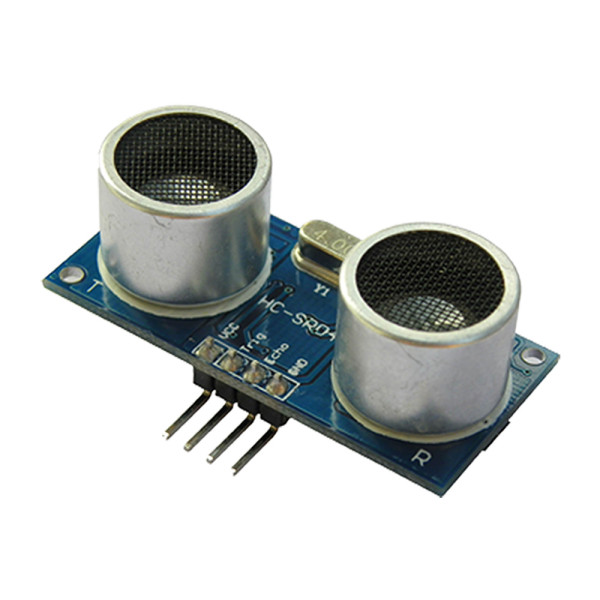
\includegraphics[width=0.4\linewidth]{HC.jpg}
  \caption{Sensor de ultrasonido HC-SR04}
\end{figure}

\subsubsection{MPU-9250 giróscopo, acelerómetro y magnetómetro}

Para poder determinar la orientación del hexapodo, se utiliza un módulo integrado de acelerómetro, giróscopo y magnetómetro MPU-9250. El magnetómetro permite determinar la orientación absoluta del robot con respecto a los polos magnéticos. 

\begin{figure}[!h]
  \centering
  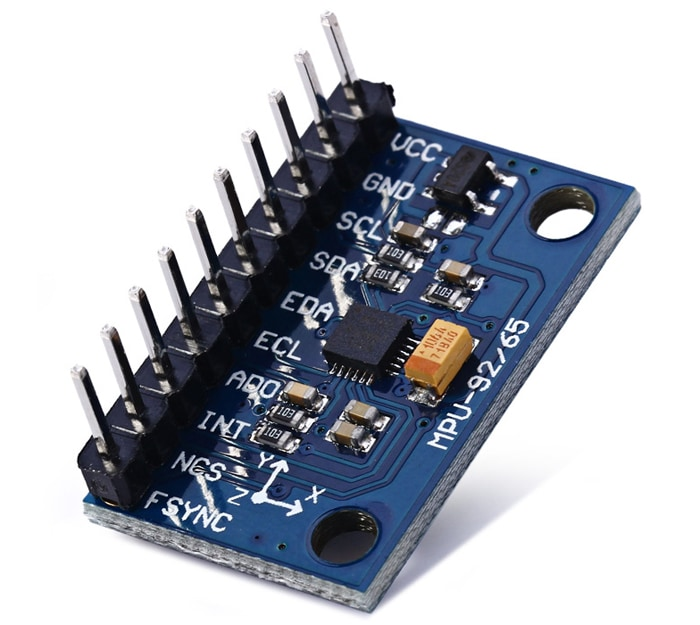
\includegraphics[width=0.4\linewidth]{MPU.jpg}
  \caption{Acelerómetro, giróscopo y magnetómetro MPU-9250}
\end{figure}


\subsubsection{Módulo de comunicación Bluetooth HC-05}

Para el control inalámbrico del robot de utiliza un módulo Bluetooth HC-05. Permite el envio de consignas para el posicionamiento del robot así como para determinar su estado en tiempo real.

\begin{figure}[!h]
  \centering
  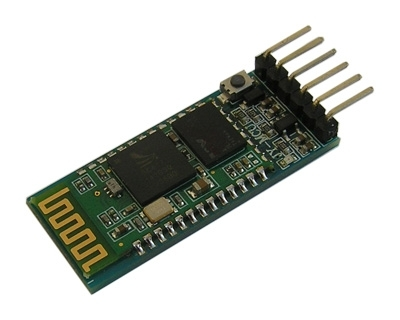
\includegraphics[width=0.4\linewidth]{BLU.jpg}
  \caption{Módulo Bluetooth HC-05}
\end{figure}

\subsubsection{Módulo GPS NEO-6}

Para determinar la posición absoluta del robot en función de la latitud y longitud terrestre se utiliza un módulo GPS NEO-6. Éste permitiría que el robot pueda planificar y realizar trayectorias entre dos puntos de forma más precisa.

\begin{figure}[!h]
  \centering
  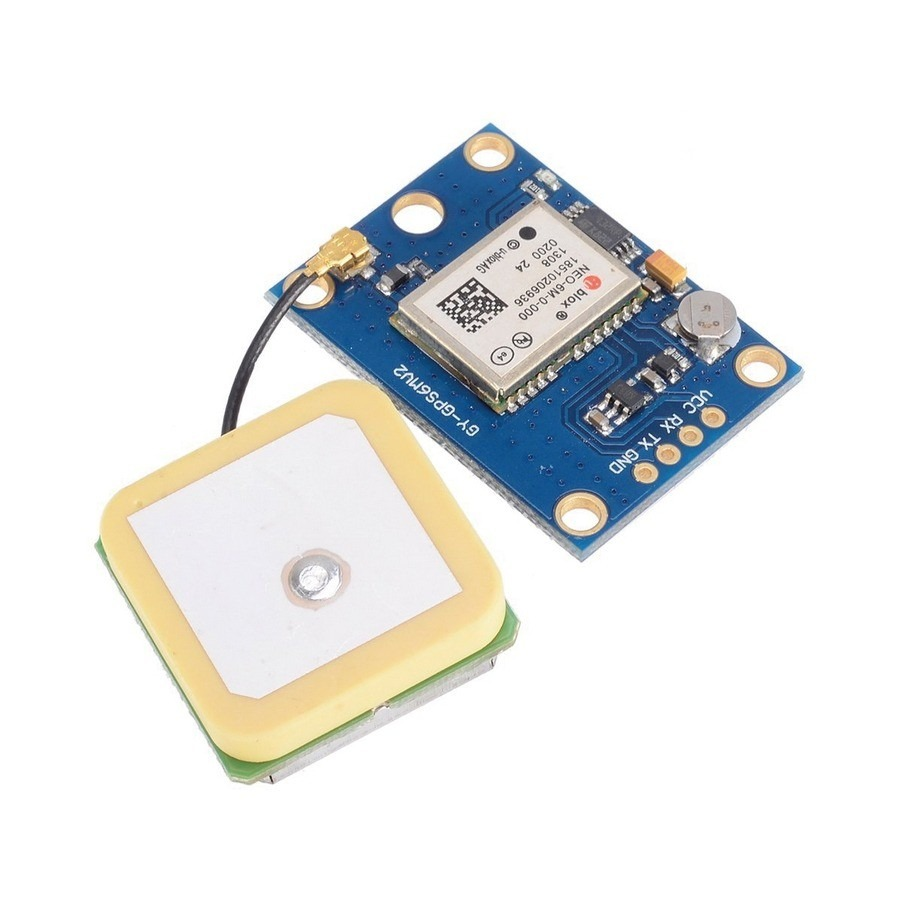
\includegraphics[width=0.4\linewidth]{GPS.jpg}
  \caption{Módulo GPS NEO-6}
\end{figure}

\subsubsection{Sensor de imágenes ov7670}

Para poder reconocer objetos y obstáculos durante las trayectorias del robot, podría utilizarse un sensor de imagenes ov7670. Se facilita de esta forma el control inalámbrico del robot.

\begin{figure}[!h]
  \centering
  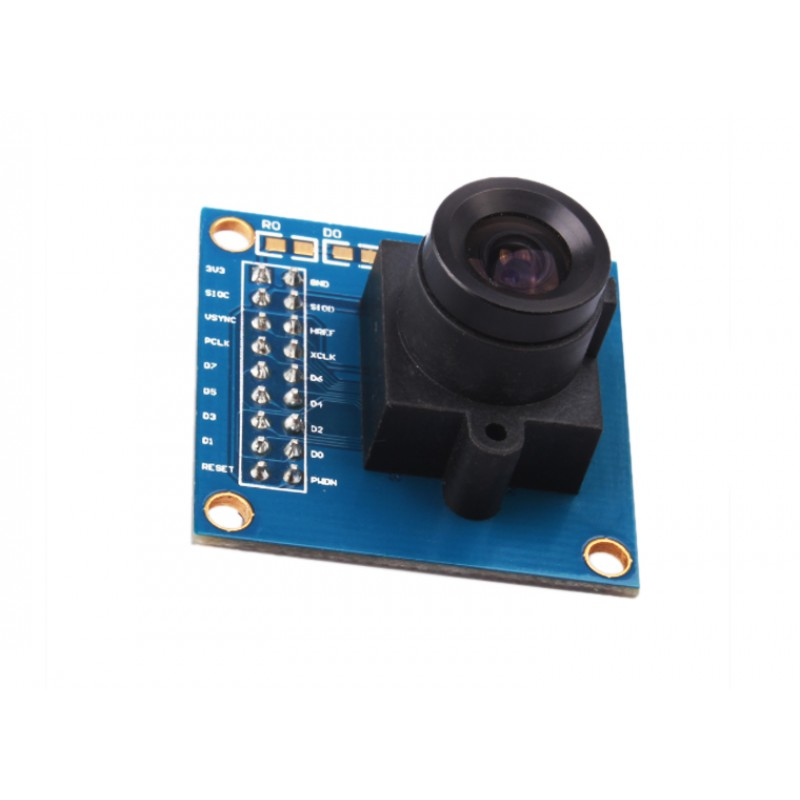
\includegraphics[width=0.5\linewidth]{OV.jpg}
  \caption{Sensor de imágenes ov7670}
\end{figure}

\subsection{Actuadores}

\subsubsection{Servo TowerPro 996r}

Para el caso de las articulaciones más desfavorables (las más alejadas del centro del robot) se utiliza Servo TowerPro 996r con un torque máximo de 11 kg.cm a 6V.

\begin{figure}[!h]
  \centering
  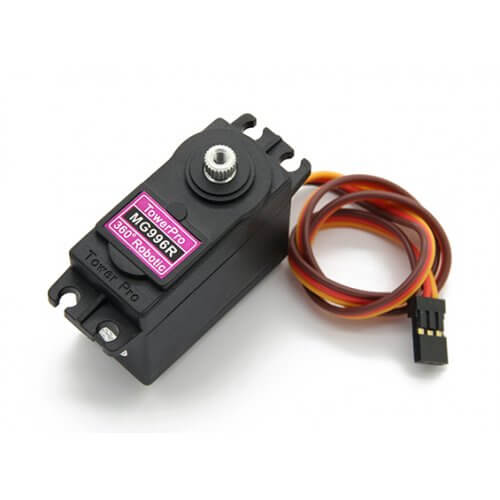
\includegraphics[width=0.5\linewidth]{MG.jpg}
  \caption{Servo TowerPro 996r}
\end{figure}

\subsubsection{Servo Futaba S3003}

Para el caso de las articulaciones menos desfavorables se utilizan motores Futaba S3003 con un torque máximo de 4.1 kg.cm a 6V.

\begin{figure}[!ht]
  \centering
  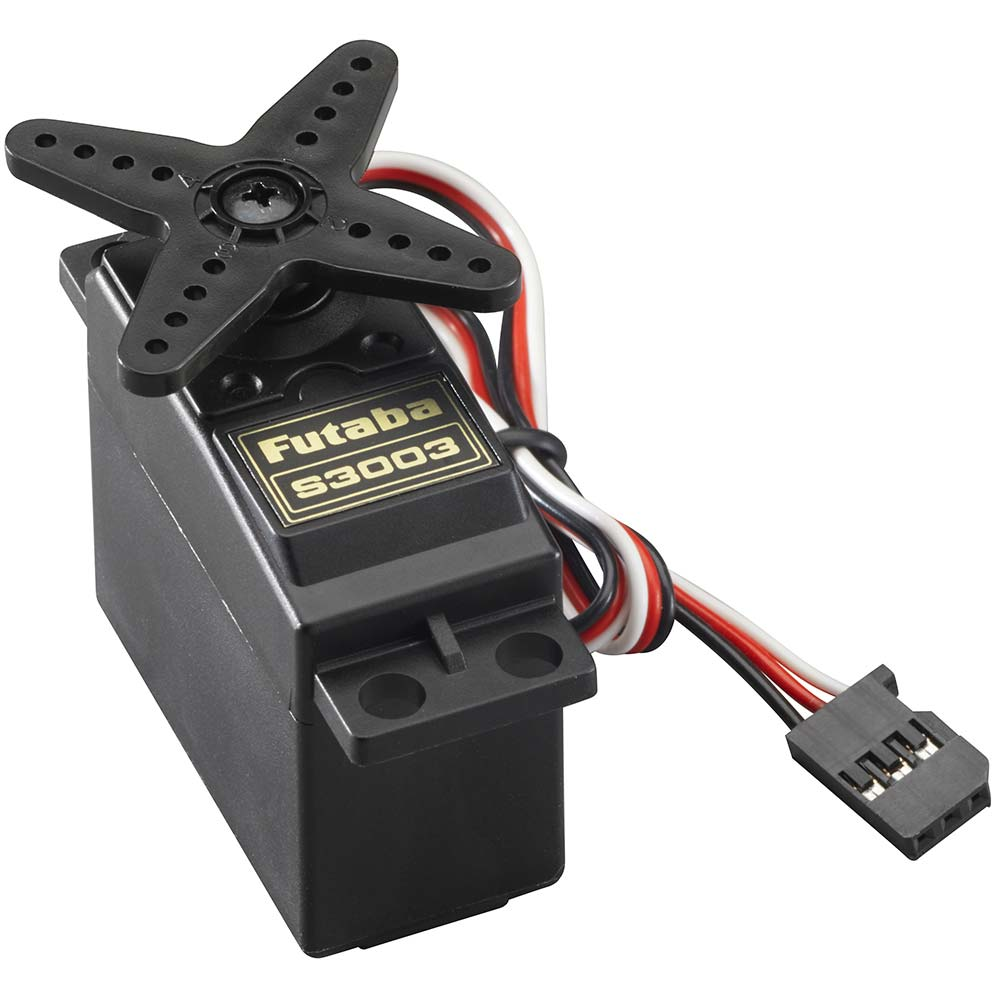
\includegraphics[width=0.5\linewidth]{FUT.jpg}
  \caption{Servo Futaba S3003}
\end{figure}



\subsection{Drivers}

\subsubsection{Controlador USC-32}

El USC-32 es un controladorde servos de 32 canales para controlar hasta 32 servos de forma simultánea. La comunicación se realiza a través de UART. El control se realiza mediante comandos que indican el servo a controlar, el ángulo y el tiempo de duración de los moviemientos.

\begin{figure}[!h]
  \centering
  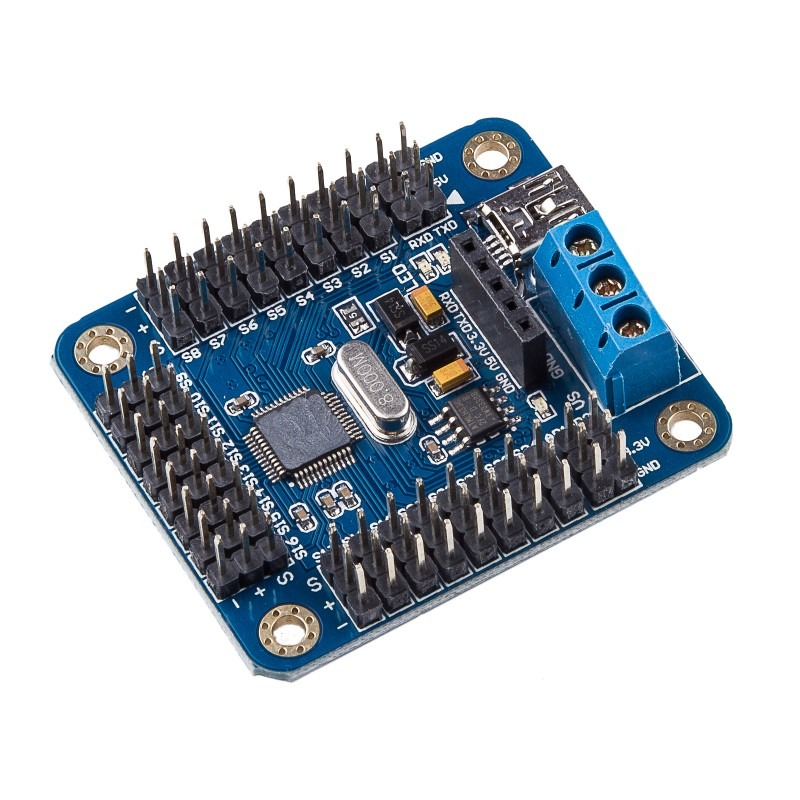
\includegraphics[width=0.5\linewidth]{Driver.jpg}
  \caption{Controlador USC-32}
\end{figure}

\end{document}
